\documentclass[a4paper]{article}
\usepackage[utf8]{inputenc}


%=-=-=-=-=-=-=-=-=-=-=-=-=-=-=-=-=-=-=-=-=-=-=-=-=-=-=-=-=-=-=-=-=-=-=-=-=-=-=-=-
% PREAMBLE
%=-=-=-=-=-=-=-=-=-=-=-=-=-=-=-=-=-=-=-=-=-=-=-=-=-=-=-=-=-=-=-=-=-=-=-=-=-=-=-=-

%%%%%%%%%%%%%%%%%%%%%%%%%%%%%%%%%%%%%%%%%%%%%%%%%%%%%%%%%%%%%%%%%%%%%
% Important styling notes
%%
% For now, to include img.jpg in img/path/to/img.jpg, just use:
% path/to/img.jpg - for details see style.tex
%=-=-=-=-=-=-=-=-=-=-=-=-=-=-=-=-=-=-=-=-=-=-=-=-=-=-=-=-=-=-=-=-=-=-=-=-=-=-=-=-
% Packages
%%
%\usepackage{fullpage} % Package to use full page
\usepackage[top=1in,bottom=1in,left=1in,right=0.7in,heightrounded]{geometry}

\usepackage{parskip}                    % Package to tweak paragraph skipping
\usepackage{amsmath}                    % standard
\usepackage{amssymb}                    % standard - Double R symbol etc.
\usepackage{hyperref}
\usepackage{amsthm}                     % standard - theorem, definition, etc.
\usepackage{multicol}                   % multiple columns for numbering
\usepackage{enumitem}                   % standard - enumerate styles
\usepackage[utf8]{inputenc}
\usepackage{scrextend}                  % indentation
\usepackage{graphicx}                   % standard - add figures
\usepackage{float}                      % standard - figure position, use [H] option
\usepackage{pifont}                     % symbols
\usepackage{gensymb}                    % degree symbol \degree
\usepackage{xcolor}                     % bg color
\hypersetup{
    colorlinks,
    linkcolor={black!50!black},
    citecolor={blue!50!black},
    urlcolor={blue!80!black}
}
\usepackage{framed}                     % bg color
\usepackage[T1]{fontenc}                % small caps
\usepackage{sectsty}                    % headings colour
\usepackage{mathtools}                  % Loads amsmath
\usepackage{amsthm,thmtools,xcolor}     % coloured theorem
\usepackage[toc,page]{appendix}         % reference to appendix
%\usepackage{titlesec}                   % change chapter, section, etc. formats
\usepackage{xifthen}                    % if, else
\usepackage{etoolbox}
% format numbering in theorem, lemma, etc. environment
\AtBeginEnvironment{theorem}{\setlist[enumerate, 1]{font=\upshape,  wide=0.5em, before=\leavevmode}}
\AtBeginEnvironment{lemma}{\setlist[enumerate, 1]{font=\upshape,  wide=0.5em, before=\leavevmode}}
\usepackage[letterspace=150]{microtype} % \textls{<letterspaced text>} % 0 <= letterspace <= 1000, 1000 = M space
\usepackage{letltxmacro}                % renew commands?
\usepackage{minted}                     % package to list code
    % otherwise minted goes off the page
    \setmintedinline{breaklines}
\usepackage{subfig}
\usepackage{eso-pic}                    % title page bg pic
\usepackage{varwidth}
\PassOptionsToPackage{svgnames}{xcolor}
\usepackage{fontawesome}                % \faQuestionCircle
\usepackage{marvosym}                   %\Pointinghand
\usepackage{mdframed}                   % easy outline frames
\usepackage[many]{tcolorbox}            % colour box for theorem styles
\usepackage{array,booktabs,calc} % table figs and text
\usepackage{comment}                    % \begin{comment}
\usepackage{fancyhdr}                   % page headings
\usepackage{mdframed}                   % boxes
\usepackage[backend=biber,sorting=none,style=ieee]{biblatex}
\usepackage{caption}
%%% caption options {
%\DeclareCaptionFont{white}{\color{white}}
\DeclareCaptionFormat{listing}{\colorbox{magenta!30!gray}{\parbox{\textwidth}{#1#2#3}}}
\captionsetup[lstlisting]{format=listing,labelfont={bf,small},textfont=small,skip=-1pt}
%%% }
\addbibresource{bibliography.bib}
\usepackage{url}
\usepackage{textcomp}
\usepackage[makeroom]{cancel}            % crossed symbols
\usepackage{algorithm}
\usepackage[noend]{algpseudocode}
\usepackage{tikz}
\usetikzlibrary{arrows.meta,positioning,quotes} % arrows and nodes in tikz
\usepackage{marginnote}
\usepackage{pgfplots}
\usepackage{pstricks-add,pst-slpe}  % for fancy tikz arrows
%\usepackage{titlesec}                   % title style
\usepackage{lmodern}                    % a font
\usepackage{titletoc} % Required for manipulating the table of contents
\usepackage{titlesec} % Allows customization of titles
\usepackage{fouriernc} % Use the New Century Schoolbook font
\usepackage{booktabs} % things in page margins
\usepackage{stmaryrd } % \varoast
\usepackage{listings} % code listings
\usepackage{longtable} % table across multiple pages
\usepackage{styles/nasm/lang}  % include custom language for NASM assembly.
\usepackage{styles/nasm/style} % include custom style for NASM assembly.



%% extra comments that I don't know where they belong:
% list of ding tags: http://willbenton.com/wb-images/pifont.pdf

%=-=-=-=-=-=-=-=-=-=-=-=-=-=-=-=-=-=-=-=-=-=-=-=-=-=-=-=-=-=-=-=-=-=-=-=-=-=-=-=-
% Colours for various things
%%


\definecolor{shadecolor}{rgb}{1.,0.933,0.96} % bg color, r,g,b <= 1
\definecolor{medium_blue}{RGB}{60,125,190}
\definecolor{dark_blue}{RGB}{25,60,85}
\definecolor{dark_red}{RGB}{77,16,16}
\definecolor{LightPink}{rgb}{0.92.,0.8,0.84} % bg color, r,g,b <= 1
\definecolor{LighterPink}{rgb}{1.,0.94,0.97} % bg color, r,g,b <= 1
\definecolor{LightestPink}{rgb}{1.,0.95,0.99} % bg color, r,g,b <= 1
\definecolor{DarkestPink}{rgb}{0.36, 0.0, 0.18}
\definecolor{DarkerPink}{rgb}{0.41, 0.0, 0.21}
\definecolor{DarkPink}{rgb}{0.55, 0.05, 0.37}
\definecolor{lightestestpink}{RGB}{255,248,252}
\definecolor{codegray}{rgb}{0.5,0.5,0.5}
\definecolor{codegrayblue}{rgb}{0.35,0.35,0.47}



%=-=-=-=-=-=-=-=-=-=-=-=-=-=-=-=-=-=-=-=-=-=-=-=-=-=-=-=-=-=-=-=-=-=-=-=-=-=-=-=-
% Define my own theorem styles
%%

% "base" styles
\declaretheoremstyle[
  headfont=\color{DarkPink}\bfseries,
  bodyfont=\itshape,
]{colored}

\declaretheoremstyle[
  headfont=\color{DarkPink}\bfseries,
  bodyfont=\normalfont,
]{colored_upright}

% theorems (corollaries, etc) themselves, inherit from my style above
% Usage:
% \begin{theorem} \end{theorem}, \begin{lemma} \end{lemma}, ...
\declaretheorem[
	numberwithin=section,
 	style=colored,
	name=\textsc{Theorem},
]{theorem}

\tcolorboxenvironment{theorem}{
  boxrule=0pt,
  boxsep=2pt,
  colback={magenta!25!white},
  colframe=DarkPink,
  enhanced jigsaw, 
  borderline west={2pt}{0pt}{DarkPink},
  sharp corners,
  before skip=5pt,
  after skip=5pt,
  breakable,
  right=0mm % for equations
}

\declaretheorem[
	numberwithin=section,
 	style=colored,
	name=\textsc{Corollary},
]{corollary}

\tcolorboxenvironment{corollary}{
  boxrule=0pt,
  boxsep=1pt,
  colback={magenta!10!white},
  colframe=DarkPink,
  enhanced jigsaw, 
  borderline west={2pt}{0pt}{DarkPink},
  sharp corners,
  before skip=5pt,
  after skip=5pt,
  breakable,
  right=0mm % for equations
}

\declaretheorem[
	numberwithin=section,
	style=colored,
	name=\textsc{Lemma},
]{lemma}

\tcolorboxenvironment{lemma}{
  boxrule=0pt,
  boxsep=1pt,
  colback={magenta!10!white},
  colframe=DarkPink,
  enhanced jigsaw, 
  borderline west={2pt}{0pt}{DarkPink},
  sharp corners,
  before skip=5pt,
  after skip=5pt,
  breakable,
  right=0mm % for equations
}

\declaretheorem[
	numberwithin=section,
	style=colored,
	name=\textsc{Definition},
]{definition}

\tcolorboxenvironment{definition}{
  boxrule=0pt,
  boxsep=1pt,
  colback={magenta!25!white},
  colframe=DarkPink,
  enhanced jigsaw, 
  borderline west={2pt}{0pt}{DarkPink},
  sharp corners,
  before skip=5pt,
  after skip=5pt,
  breakable,
  right=0mm % for equations
}

\declaretheorem[
	numberwithin=section,
  	style=colored,
  	name=\textsc{Example},
]{exmp}

\declaretheorem[
	numberwithin=section,
  	style=colored,
  	name=\textsc{Solution},
]{soln}

%%% code listings
\lstdefinestyle{code1}{
    backgroundcolor=\color{lightestestpink},   
    commentstyle=\color{codegrayblue},
    keywordstyle=\color{DarkerPink},
    numberstyle=\tiny\color{codegray},
    stringstyle=\color{black!40!cyan},
    basicstyle=\small\ttfamily,
    breakatwhitespace=false,
    breaklines=true,        
    captionpos=t,             
    keepspaces=true,        
    numbers=left,           
    numbersep=5pt,
    showspaces=false, 
    showstringspaces=false,
    showtabs=false,
    tabsize=4
}

\lstset{style=code1}

%=-=-=-=-=-=-=-=-=-=-=-=-=-=-=-=-=-=-=-=-=-=-=-=-=-=-=-=-=-=-=-=-=-=-=-=-=-=-=-=-
% Headers (size, font, colour)
%%




\makeatletter
\renewcommand{\@seccntformat}[1]{\llap{\textcolor{DarkestPink}{\csname the#1\endcsname}\hspace{1em}}}                    
\renewcommand{\section}{\@startsection{section}{1}{\z@}
{-4ex \@plus -1ex \@minus -.4ex}
{1ex \@plus.2ex }
{\normalfont\large\sffamily\bfseries\textcolor{DarkestPink}}}
\renewcommand{\subsection}{\@startsection {subsection}{2}{\z@}
{-3ex \@plus -0.1ex \@minus -.4ex}
{0.5ex \@plus.2ex }
{\normalfont\sffamily\bfseries\textcolor{DarkestPink}}}
\renewcommand{\subsubsection}{\@startsection {subsubsection}{3}{\z@}
{-2ex \@plus -0.1ex \@minus -.2ex}
{.2ex \@plus.2ex }
{\normalfont\small\sffamily\bfseries\textcolor{DarkestPink}}}                        


%=-=-=-=-=-=-=-=-=-=-=-=-=-=-=-=-=-=-=-=-=-=-=-=-=-=-=-=-=-=-=-=-=-=-=-=-=-=-=-=-
% Numberings, counters and spacings
%%
\numberwithin{equation}{section} % section number in eq/s
\setlength{\jot}{7pt} % spacing in split, gathered env/s



%% Custom examples
%% Output - Example 1,2,...
\newcounter{example}
\newenvironment{example}[1][]{\refstepcounter{example}\par\medskip
   \textbf{Example~\theexample. #1} \rmfamily}{\medskip}
%%%%%%%%%%%% End of unused %%%%%%%%%%%%



%=-=-=-=-=-=-=-=-=-=-=-=-=-=-=-=-=-=-=-=-=-=-=-=-=-=-=-=-=-=-=-=-=-=-=-=-=-=-=-=-
% Paths
%%
\graphicspath{ {./img/} } % figures' path - can look up files directly from there


%=-=-=-=-=-=-=-=-=-=-=-=-=-=-=-=-=-=-=-=-=-=-=-=-=-=-=-=-=-=-=-=-=-=-=-=-=-=-=-=-
% User defined macros (math mode)
%%


% Curly braces under text. Usage: \myunderbrace{upper}{lower}
\newcommand{\myunderbrace}[2]{\mathrlap{\underbrace{\phantom{#1}}_{#2}} #1}
\newcommand{\setR}{\mathbb{R}} % \ouble R
\newcommand{\setRn}{\mathbb{R}^n} %  double R^n
\newcommand{\setN}{\mathbb{N}} % double N
\newcommand{\setZ}{\mathbb{Z}} % double Z
\let\oldemptyset\emptyset
\let\emptyset\varnothing % nice - looking empty set symbol
\newcommand{\fancyN}{\mathcal{N}} % null space
\newcommand{\fancyR}{\mathcal{R}} % range

\newcommand{\bx}{\textbf{x}}
\newcommand{\by}{\textbf{y}}
\newcommand{\bb}{\textbf{b}}
\newcommand{\bA}{\textbf{A}}
\newcommand{\bB}{\textbf{B}}
\newcommand{\bI}{\textbf{I}}
% double bars as in norm
\newcommand{\norm}[1] {\lVert #1 \rVert} 
\newcommand{\trans}[1]{#1^{\top}}

\newcommand{\mean}[1]{\bar{#1}}
\newcommand{\var}{\sigma^2}

\newcommand{\partdevx}[1]{\frac{\partial #1}{\partial x}}
\newcommand{\partdevxx}[1]{\frac{\partial #1}{\partial x}}
\newcommand{\partdevxn}[1]{\frac{\partial^n #1}{\partial x^n}}
\newcommand{\partdevy}[1]{\frac{\partial #1}{\partial x}}
\newcommand{\partdevyy}[1]{\frac{\partial #1}{\partial y}}
\newcommand{\partdevyn}[1]{\frac{\partial^n #1}{\partial y^n}}

% text above = symbol
\newcommand{\overeq}[1]{\ensuremath{\stackrel{#1}=}} 
\newcommand{\greatersmaller}{%
  \mathrel{\ooalign{\raisebox{.6ex}{$>$}\cr\raisebox{-.6ex}{$<$}}}
} % greater and smaller symbols on top of each other, same line

%=-=-=-=-=-=-=-=-=-=-=-=-=-=-=-=-=-=-=-=-=-=-=-=-=-=-=-=-=-=-=-=-=-=-=-=-=-=-=-=-
% User defined macros (non math)

\newcommand{\qedblack}{$\hfill\blacksquare$} % black square end of line
\newcommand{\qedwhite}{\hfill \ensuremath{\Box}} % white square end of line
\newcommand{\hquad}{\hskip0.5em\relax}% half quad space
%\newcommand{\TODO}{\textcolor{red}{\bf TODO!}\;}

\newcommand{\TODO}[1][]{%
    \ifthenelse{\equal{#1}{}}{\textcolor{red}{\bf TODO!}\;}{\textcolor{red}{\textbf {TODO:} #1}\; }%
}
\newcommand{\B}[1]{\textbf{\textup{#1}}} % bold and upright
\renewcommand{\labelitemi}{\scriptsize$\textcolor{DarkPink}{\blacksquare}$} % itemize - squares instead of bullets
\newcommand{\emphasis}[1]{\textls{#1}}

\LetLtxMacro{\originaleqref}{\eqref}
\renewcommand{\eqref}{Eq.~\originaleqref}
\renewcommand*{\eqref}[1]{Eq.~\originaleqref{#1}}





% background images
%%%%%%%
\newcommand\BackgroundPic{%
\put(0,0){%
\parbox[b][\paperheight]{\paperwidth}{%
\vfill
%\centering

\includegraphics[width=0.125\paperwidth,height=\paperheight,%
]{img/background_02.png}% use ,keepaspectratio
\vfill
}}}
%%%%%%%
% end of background image
%%%%%%%%%%%%%% my own frame
\newmdenv[topline=false,bottomline=false]{leftrightbox}
%%%%%%%%%%%%% end
%%%%%%%%%%%%% my own comment
\newcommand{\mycomment}[1]{\begin{leftrightbox}\Pointinghand~\textbf{Comment:}~#1 \end{leftrightbox}}
%%%%%%%%%%%%% end
% my custom note https://tex.stackexchange.com/questions/301993/create-custom-note-environment-with-tcolorbox
\newmdenv[
    topline=false,
    bottomline=false,
    rightline=false,
    innerrightmargin=0pt
]{siderule}
\newenvironment{mynote}%
    {\begin{siderule}\textbf{\Pointinghand~Note:}}
    {\end{siderule}}
%%%%%%%%%%%%% my own box
\newcommand{\boxone}[1]{\begin{tcolorbox}[colback = LighterPink,colframe=LightPink]
#1
\end{tcolorbox}}
%%%%%%%%%%%%% end

\let\oldemptyset\emptyset
\let\emptyset\varnothing
%algorithmic
\algdef{SE}[DOWHILE]{Do}{doWhile}{\algorithmicdo}[1]{\algorithmicwhile\ #1}%






\begin{document}
%=-=-=-=-=-=-=-=-=-=-=-=-=-=-=-=-=-=-=-=-=-=-=-=-=-=-=-=-=-=-=-=-=-=-=-=-=-=-=-=-
% GLOBAL STYLES (DOCUMENT SCOPE)
%=-=-=-=-=-=-=-=-=-=-=-=-=-=-=-=-=-=-=-=-=-=-=-=-=-=-=-=-=-=-=-=-=-=-=-=-=-=-=-=-
% caption: Figure 1 -> <bold> Fig. 1 </bold>
\captionsetup[figure]{labelfont={bf},labelformat={default},labelsep=period,name={Fig.}}


%=-=-=-=-=-=-=-=-=-=-=-=-=-=-=-=-=-=-=-=-=-=-=-=-=-=-=-=-=-=-=-=-=-=-=-=-=-=-=-=-
% TITLE PAGE
%=-=-=-=-=-=-=-=-=-=-=-=-=-=-=-=-=-=-=-=-=-=-=-=-=-=-=-=-=-=-=-=-=-=-=-=-=-=-=-=-
%%%%%%%%%%%%%%%%%%%%%%%%%%%%%%%%%%%%%%%%%
% Formal Book Title Page
% LaTeX Template
% Version 2.0 (23/7/17)
%
% This template was downloaded from:
% http://www.LaTeXTemplates.com
%
% Original author:
% Peter Wilson (herries.press@earthlink.net) with modifications by:
% Vel (vel@latextemplates.com)
%
% License:
% CC BY-NC-SA 3.0 (http://creativecommons.org/licenses/by-nc-sa/3.0/)
% 
% This template can be used in one of two ways:
%
% 1) Content can be added at the end of this file just before the \end{document}
% to use this title page as the starting point for your document.
%
% 2) Alternatively, if you already have a document which you wish to add this
% title page to, copy everything between the \begin{document} and
% \end{document} and paste it where you would like the title page in your
% document. You will then need to insert the packages and document 
% configurations into your document carefully making sure you are not loading
% the same package twice and that there are no clashes.
%
%%%%%%%%%%%%%%%%%%%%%%%%%%%%%%%%%%%%%%%%%

%----------------------------------------------------------------------------------------
%	PACKAGES AND OTHER DOCUMENT CONFIGURATIONS
%----------------------------------------------------------------------------------------



%----------------------------------------------------------------------------------------
%	TITLE PAGE
%----------------------------------------------------------------------------------------



\begin{titlepage} % Suppresses headers and footers on the title page

	\centering % Centre everything on the title page
	
	\scshape % Use small caps for all text on the title page
	
	\vspace*{\baselineskip} % White space at the top of the page
	
	%------------------------------------------------
	%	Title
	%------------------------------------------------
	
	\rule{\textwidth}{1.6pt}\vspace*{-\baselineskip}\vspace*{2pt} % Thick horizontal rule
	\rule{\textwidth}{0.4pt} % Thin horizontal rule
	
	\vspace{0.75\baselineskip} % Whitespace above the title
	
	{\LARGE COMPUTER VISION NOTES\\ \Large OBJECT LOCALISATION AND TRACKING\\} % Title
	
	\vspace{0.75\baselineskip} % Whitespace below the title
	
	\rule{\textwidth}{0.4pt}\vspace*{-\baselineskip}\vspace{3.2pt} % Thin horizontal rule
	\rule{\textwidth}{1.6pt} % Thick horizontal rule
	
	\vspace{2\baselineskip} % Whitespace after the title block
	
	%------------------------------------------------
	%	Subtitle
	%------------------------------------------------
	My personal notes on
	
	\vspace*{3\baselineskip} % Whitespace under the subtitle
	
	Object Localisation Techniques; Colour Matching, Mean Shift Tracking, Optical Flow, Lukas Kanade 
	
	\vspace*{3\baselineskip} % Whitespace under the subtitle
	
	%------------------------------------------------
	%	Editor(s)
	%------------------------------------------------
	
	By
	
	\vspace{0.5\baselineskip} % Whitespace before the editors
	
	{\normalfont \Large \mintinline{latex}{0xLeo} (\url{github.com/0xleo}) \\} % Editor list
	
	\vspace{0.5\baselineskip} % Whitespace below the editor list
	
	%\textit{The University of California \\ Berkeley} % Editor affiliation
	
	\vfill % Whitespace between editor names and publisher logo
	
	%------------------------------------------------
	%	Publisher
	%------------------------------------------------
	
	
	\vspace{0.3\baselineskip} % Whitespace under the publisher logo
	
	\today % Date
	
	{DRAFT X.YY} % Draft version
	{\\Missing: \ldots}

\end{titlepage}

%----------------------------------------------------------------------------------------

%\maketitle



%=-=-=-=-=-=-=-=-=-=-=-=-=-=-=-=-=-=-=-=-=-=-=-=-=-=-=-=-=-=-=-=-=-=-=-=-=-=-=-=-
% MAIN DOCUMENT
%=-=-=-=-=-=-=-=-=-=-=-=-=-=-=-=-=-=-=-=-=-=-=-=-=-=-=-=-=-=-=-=-=-=-=-=-=-=-=-=-
\newpage
\tableofcontents
\newpage



%------------------------------ New section ------------------------------%
\section{Bresenhma's line drawing algorithm}


\subsection{Introduction}
Bresenham's line drawing algorithm was proposed in 1962. It takes as input two points and draws a line between in a discrete 2D grid. It decides either to draw or not to draw a pixel by traversing them in a certain way.


% https://cse.iitkgp.ac.in/~pb/pb-graphics-2018.pdf
% https://www.cs.helsinki.fi/group/goa/mallinnus/lines/bresenh.html
% http://www.csc.villanova.edu/~mdamian/Past/csc8470sp15/notes/Rasterization.pdf
% https://blog.mbedded.ninja/programming/algorithms-and-data-structures/bresenhams-line-algorithm/
% https://www.youtube.com/watch?v=y_SPO_b-WXk
\subsection{Assumptions}

\begin{itemize}
	\item All pixels are sampled in a discrete 2D lattice.
	\item The algorithm does not draw any colours -- it simple decides whether to draw a pixel or not.
	\item The line generated does not contain any holes. All line pixels must be 8-connected and each column ($x$) must correspond to a row ($y$). 
\end{itemize}
To understand its advantages, we'll try to derive the algorithm.


\subsection{Deriving the algorithm}
\subsubsection{First attempt; a naive implementation}

Given two points $(x_1,y_1), \; (x_2,y_2)$, a naive first implementation is to iterate over all $x$'s and find their $y$'s as follows:
\begin{equation}
	y = \textup{round}(m\cdot x + b), \quad m = \frac{y_2 - y_1}{x_2 - x_1} 
\end{equation}
Translated to C:
\begin{verbatim}
#include <math.h>

/* Draw a line in a naive way assuming x1 < x2 */
void gfx_naive_line(int x1, int y1, int x2, int y2)
{
    // y = mx + b
    float m = (y2 - y1)/(x2 - x1);
    float b = y1 - m*x1; 
    int x;
    int y;
    for (x = x1; x < x2; x++)
    {
        y = round(m*x + b);
        gfx_point(x,y);
    }
}
\end{verbatim}
The drawback of this approach is that for each pixel it uses 2 floating point operations (plus rounding, which is expensive);
\begin{itemize}
	\item Multiplication \texttt{m*x}
	\item Addition of \texttt{m*c} with \texttt{b}
	\item For now, we'll only be implementing the algorithm in the first octant ($0\deg$ to $45\deg$ with $x$ axis), i.e. assume that for the slope of the line $0 \leq m \leq 1$.
\end{itemize}
The cost of these operations adds up when 100s of pixels are drawn every time. Floating point operations are relatively expensive for CPUs and replacing them with integer arithmetic is often a significant optimisation. Bresenham's algorithm fully relies on integer operations.


\subsubsection{Bresenham's line drawing algorithm idea}
Consider drawing a line on the first octant (\ref{fig:octants}) ($0\deg$ to $45\deg$)of the 2D discrete lattice. The remaining 7 octants will be addressed later. Therefore the main constraint imposed is
\begin{equation}
	0 \leq m \leq 1,\quad m = \frac{y_2-y_1}{x_2-x_1} 
	\label{eq:slope_leq_1}
\end{equation}
, i.e. $x_2 - x_1 \geq y_2 - y_1$.
\begin{figure}[H]
	\centering
	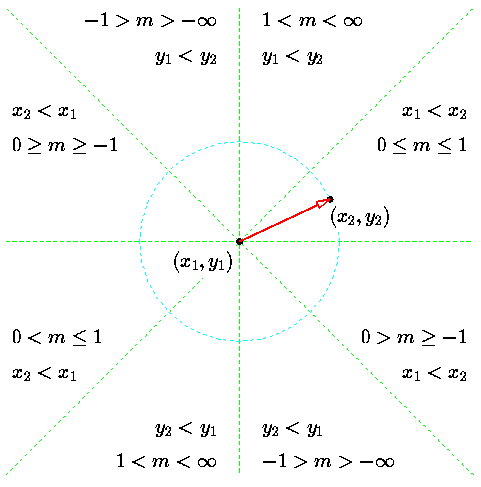
\includegraphics[height=5.5cm]{img/octants.png}
	\caption{The 8 octants and their slopes \cite{mallinus}.}
	\label{fig:octants}
\end{figure}

Let's say we have plotted a pixel $(x,y)$ of the rasterised line. Because of the constraint in \eqref{eq:slope_leq_1}, the next pixel can be either East ($x+1,y$) or North-East ($x+1,y+1$). When the line is drawn in 2D, for each step from $x$ to $x+1$, we have to find whether $y$ or $y+1$ is closest to the $y$ (floating) of the line. To do that, we increment $y$ by the slope $m$ (def'n of slope) and have to determine whether $y+m$ is above or below the midway $y+0.5$  between $y, \ y+1$ (Fig. \ref{fig:grid_line_1st_octant}).

\begin{multicols}{2}
	\begin{figure}[H]
		\centering
		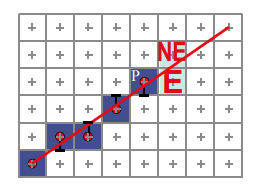
\includegraphics[height=4cm]{img/next_pixel_n_ne.png}
		\caption{At every update of pixel $(x,y)$, we choose between the E and NE neighbour \cite{mdamian}.}
		\label{fig:}
	\end{figure}
\columnbreak
	\begin{figure}[H]
	\centering
	

%\usepackage{tikz}
\usetikzlibrary{calc}


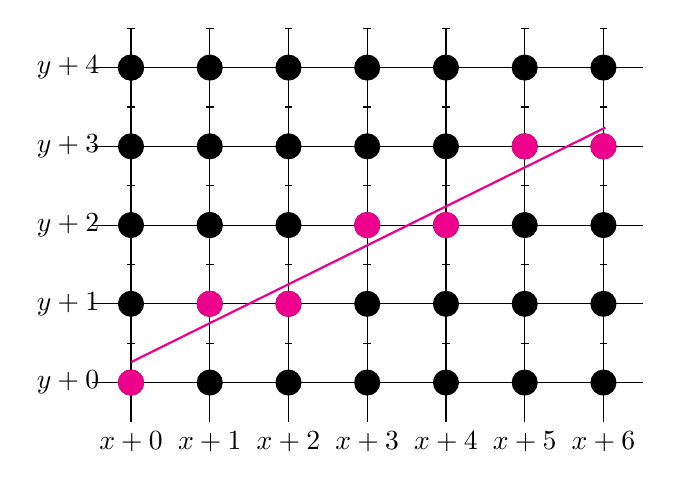
\begin{tikzpicture}
	\begin{scope}
		
\tikzset{dot/.style={fill=black,circle}}

%\foreach\l[count=\y] in {E,...,A}
\foreach \y in {0,1,...,4}
{
\draw (0.5,\y+1) -- (7.5,\y+1);
\node at (0.2,\y+1){$y + \y$};
}

\foreach \x in {0,1,...,6}
{
\draw (\x+1,0.5) -- (\x+1,5.5);
\node at (\x+1, 0.25){$x + \x$};
}

\foreach \x in {1,2,...,7}
{
	\foreach \y in {1,2,...,5}
	{
		\node[dot] at (\x,\y){};
		\draw(\x-0.05,\y+0.5) --(\x+0.05,\y+0.5);
	}
}


\node(p1)[dot] at (1,5){};
\node(p2)[dot] at (2,3){};

% the actual line
\node(st) at (0.88,1.2){};
\node(end) at (7.15,4.3){};
\draw [magenta, thick] (st) -- (end);

% draw its Bresenham points
\node[dot,magenta] at (1,1){};
\node[dot,magenta] at (2,2){};
\node[dot,magenta] at (3,2){};
\node[dot,magenta] at (4,3){};
\node[dot,magenta] at (5,3){};
\node[dot,magenta] at (6,4){};
\node[dot,magenta] at (7,4){};

	\end{scope}
\end{tikzpicture}

	\caption{The nodes represent pixel centres and the segments the midway $y$ between neighbouring pixels. Nodes in magenta represent where the line will be drawn in the 2D discrete space.}
	\label{fig:grid_line_1st_octant}
\end{figure}


\end{multicols}{2}

\subsubsection{Bresenham's line drawing at 1st octant; the derivation}

Because we plot the original line in a discrete grid given a resolution, it will almost never cross a discrete point. Therefore it will always be at some error $\epsilon$ above or below the nearest discrete $y$. For the error \cite{mallinus},
\begin{equation}
	-0.5 \leq \epsilon <0.5
\end{equation}
The $y_{actual}$ ordinate of the line is then given by $y_{actual} = y+\epsilon$. In moving from $x$ to $x+1$ we increase the value of the true (mathematical) $y$-ordinate by an amount equal to the slope $m$ (Fig. \ref{fig:error_diagram}).
\begin{figure}[H]
	\centering
	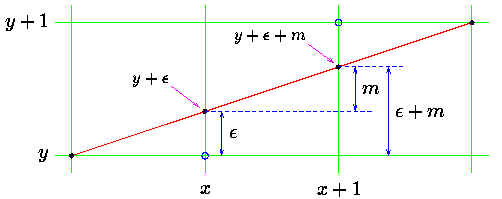
\includegraphics[height=4.5cm]{img/error_diagram.png}
	\caption{The error at each pixel during the update \cite{mallinus}.}
	\label{fig:error_diagram}
\end{figure}
From the plot in Fig. \ref{fig:error_diagram}, it is clear after the transition $x\rightarrow x+1$, if 
\begin{gather*}
	y + \epsilon + m < y+  0.5 \Rightarrow\\
	\epsilon + m < 0.5
\end{gather*}
, then we move East ($x+1,y$) to represent the line. Else we move North-East ($x+1,y+1$). We make this decision to minimise the total error between what gets drawn on the display and the actual values.

However, after $x\rightarrow x+1$ the error gets updated too from $\epsilon$ to $\epsilon_{new}$. We know that the error the distance of the mathematical line to the nearest $y$-ordinate of the grid, i.e. either $y$ or $y+1$. In case $(x+1,y)$, the new error is given by \cite{mallinus} (Fig. \ref{fig:error_diagram})
\begin{equation}
	\epsilon_{new} \leftarrow (y+\epsilon + m) - y  = \epsilon + m
\end{equation}
Else, if ($x+1,y+1$) was chosen
\begin{equation}
	\epsilon_{new} \leftarrow (y+\epsilon + m) - (y+1) = \epsilon + m -1	
\end{equation}
Therefore a first implementation of the line drawing algorithm so far is below. Note that it still uses floating point which must be eliminated. Note also that for the algorithm to be consistent with the idea developed thus far, it is assumed that $(x_1,y_1)$ is closer to the origin than $(x_2,y_2)$.
\begin{algorithm}[H]
\caption{Line drawing with FP operations.}
\label{alg:line_drawing_fp}
\begin{algorithmic}[1]
\Procedure{Line-Drawing-FP} {$x_1,\; y_1,\; x_2,\; y_2$} 
	\State $m \leftarrow \frac{y_2-y_1}{x_2-x_1} $
	\State $\epsilon \leftarrow 0, \; y\leftarrow y_1$ \Comment{$\epsilon, \; y$ are all we keep track of.}
\For{$x=x_1,\ldots,x_2$} 
	\State DrawPixel($x,\; y$)
	\If{$\epsilon + m < 0.5$}
		\State $\epsilon \leftarrow \epsilon + m$ \Comment{Move E; don't change $y$}
	\Else
		\State $\epsilon \leftarrow \epsilon + m - 1$ \Comment{Move NE}
		\State $y\leftarrow y + 1$
	\EndIf
\EndFor
\EndProcedure
\end{algorithmic}
\end{algorithm}
To optimise the algorithm, we must convert the following to integer operations
\begin{gather*}
\epsilon + m < 0.5 \tag{1}	\\
	\epsilon \leftarrow \epsilon + m \tag{2}\\
	\epsilon \leftarrow \epsilon + m - 1 \tag{3}
\end{gather*}
Plugging in $m=\Delta x/\Delta y = (y_2-y_1)/(x_2-x_1)$, Eq. (1) becomes
\[	
	2\underbrace{\epsilon\Delta x}_{\epsilon'}  + 2\Delta y < \Delta x \tag{1'}
\]
Eq. (2) and (3) become respectively
\begin{gather*}
	\underbrace{\epsilon\Delta x}_{} \leftarrow \underbrace{\epsilon \Delta x}_{} + \Delta y \tag{2'}\\
	\underbrace{\epsilon\Delta x}_{} \leftarrow \underbrace{\epsilon \Delta x}_{} + \Delta y - \Delta x \tag{3'}\\
\end{gather*}
\marginnote{Algo stated assuming $0\leq m \leq 1$ and $x_1<x_2$.}.The quantity $\epsilon\Delta x$ appears in all Eq. (1'), (2'), (3') therefore we let $\epsilon' := \epsilon \Delta x$. The algorithm we have arrived in is \textit{Bresenham's for the 1st octant}. It is written in integer arithmetic as follows:
\begin{algorithm}[H]
\caption{Bresenham's line drawing -- 1st octant.}
\label{alg:bres_1st_oct}
\begin{algorithmic}[1]
\Procedure{Bresenham-1st-Octant} {$x_1,\; y_1,\; x_2,\; y_2$} 
	\State $\Delta x \leftarrow x_2 - x_1$
	\State $\Delta y \leftarrow y_2 - y_1$
	\State $\epsilon' \leftarrow 0, \; y\leftarrow y_1$ \Comment{$\epsilon', \; y$ are all we keep track of.}
	\If {$0 \leq \frac{\Delta y}{\Delta x} < 1 $}
\For{$x=x_1,\ldots,x_2$} 
	\State DrawPixel($x,\; y$)
	\If{$2(\epsilon'  + \Delta y) < \Delta x$}
		\State $\epsilon' \leftarrow \epsilon' + \Delta y$ \Comment{Move E; don't change $y$}
	\Else
		\State $\epsilon' \leftarrow \epsilon' + \Delta y - \Delta x$ \Comment{Move NE}
		\State $y\leftarrow y + 1$
	\EndIf
\EndFor
\EndIf
\EndProcedure
\end{algorithmic}
\end{algorithm}
This version is particularly efficient not only due to integer arithmetic but as multiplication by 2 can be implemented as left bit shifting. We can of course move the update $\epsilon' \leftarrow \epsilon'+\Delta y$ before the if-else block to end up with only one if for slightly more conciseness. 


\subsubsection{Bresenham's line drawing algorithm in octant 2}

We now address the case of drawing a line with slope $1 \leq m < \infty$, i.e. one that spans at the 2nd octant (Fig. \ref{fig:octants}). Note that a line $(l1): \; y=mx+b$ with slope $0 \leq m < 1$ in the first octant is symmetric w.r.t to $y=x$ to the line $(l2): \; x=my+b \Leftrightarrow y = \frac{x}{m} - \frac{b}{m}$ (e.g. Fig. \ref{fig:symmetric_lines_octants_1_2}). If $(x_0,y_0)\in(l1)$ then $(y_0,x_0)\in (l2)$. Therefore to rasterise $(l2)$ we can apply Alg. \ref{alg:bres_1st_oct} on it modified by swapping $x$ with $y$ and $\Delta x$ with $\Delta y$. Don't forget the ordinate condition for the 2nd octant, which is $y_1<y_2$.
\begin{figure}[H]
	\centering
	\usetikzlibrary{calc}


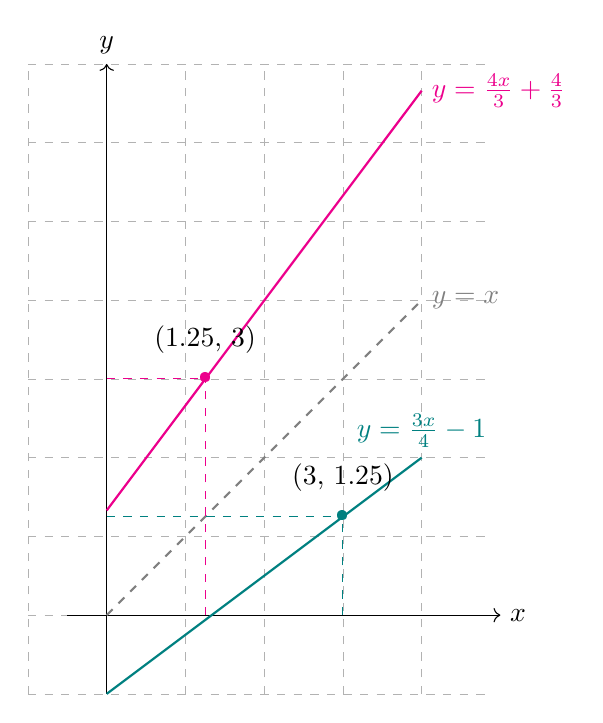
\begin{tikzpicture}
	\begin{scope}
\draw[help lines, color=gray!60, dashed] (-1,-1) grid (4.9,7);
\draw[->] (-0.5,0)--(5,0) node[right]{$x$};
\draw[->] (0,-1)--(0,7) node[above]{$y$};
\draw[thick,teal] (0,-1)--(4,2) node[above]{$y=\frac{3x}{4}-1$};
\draw[thick,magenta] (0,1.33)--(4,6.66) node[right]{$y= \frac{4x}{3}+ \frac{4}{3}$};
\draw[thick,gray,dashed] (0,0)--(4,4) node[right]{$y=x$};

\node [magenta, label={(1.25,$\ $3)}] at (1.25,3) {\textbullet};
\node [teal, label={(3,$\ $1.25)}] at (3, 1.25) {\textbullet};

\draw[thick,thin,teal,dashed] (3,0)--(3,1.25) node[right]{};
\draw[thick,thin,teal,dashed] (0,1.25)--(3,1.25) node[right]{};

\draw[thick,thin,magenta,dashed] (1.25,0)--(1.25,3) node[right]{};
\draw[thick,thin,magenta,dashed] (0,3)--(1.25,3) node[right]{};

	\end{scope}
\end{tikzpicture}

	\caption{Two lines in the first two octants symmetric about line $y=x$.}
	\label{fig:symmetric_lines_octants_1_2}
\end{figure}
\begin{algorithm}[H]
\caption{Bresenham's line drawing -- 2nd octant.}
\label{alg:bres_2nd_oct}
\begin{algorithmic}[1]
\Procedure{Bresenham-2nd-Octant} {$x_1,\; y_1,\; x_2,\; y_2$} 
	\State $\Delta x \leftarrow x_2 - x_1$
	\State $\Delta y \leftarrow y_2 - y_1$
	\State $\epsilon' \leftarrow 0, \; x\leftarrow x_1$ \Comment{$\epsilon', \; y$ are all we keep track of.}
	\If {$1\leq \frac{\Delta y}{\Delta x} $ and $y_1<y_2$}
		\For{$y=y_1,\ldots,y_2$} 
			\State DrawPixel($x,\; y$)
			\If{$2(\epsilon'  + \Delta x) < \Delta y$}
				\State $\epsilon' \leftarrow \epsilon' + \Delta x$ 
			\Else
				\State $\epsilon' \leftarrow \epsilon' + \Delta x - \Delta y$ 
				\State $x\leftarrow x + 1$
			\EndIf
		\EndFor
	\EndIf
\EndProcedure
\end{algorithmic}
\end{algorithm}
Octants 1 and 2 (quadrant 1) have been addressed. To complete the algorithm in the remaining 6 octants, observe that quadrant 2 (octants 3,4) is symmetric with quadrant 1 w.r.t the $y$ axis. Quadrant 3 (octants 5, 6) is symmetric with 1 w.r.t $x$ and $y$ axes, and quadrant 4 is symmetric with 1 w.r.t the $x$ axis.


\subsubsection{Bresenham's line drawing algorithm in octants 3 and 4}

Octants 3 and 4 are symmetric w.r.t the $y$ axis to octants 2 and 1 respectively. Therefore to derive their line drawing we start with Alg. \ref{alg:bres_2nd_oct} and \ref{alg:bres_1st_oct} respectively and substitute $(-x,y) \leftarrow (x,y)$, $\Delta x \leftarrow -\Delta x$. Therefore the line drawing for those octants is formulated as follows, renaming the error $\epsilon'$ to $\epsilon$ for simplicity.
\begin{algorithm}[H]
\caption{Bresenham's line drawing -- 2nd quadrant.}
\label{alg:bres_2nd_qd}
\begin{algorithmic}[1]
\Procedure{Bresenham-2nd-Quadrant} {$x_1,\; y_1,\; x_2,\; y_2$} 
	\State $\Delta x \leftarrow x_2 - x_1$
	\State $\Delta y \leftarrow y_2 - y_1$
	\State $\epsilon \leftarrow 0, \; y\leftarrow y_1$ 
	\If {$\frac{\Delta y}{\Delta x} < -1$ and $y_1 < y_2$} \Comment{This is the 3rd octant (2nd octant mirror w.r.t $y$ axis)}
		\For{$y=y_1,\ldots,y_2$} 
			\State DrawPixel($x,\; y$)
			\If{$2(\epsilon  - \Delta x) < \Delta y$}
				\State $\epsilon \leftarrow \epsilon - \Delta x$ 
			\Else
				\State $\epsilon \leftarrow \epsilon - \Delta x - \Delta y$ 
				\State $x\leftarrow x - 1$
			\EndIf
		\EndFor
	\ElsIf {$0 \leq \frac{\Delta y}{\Delta x} < -1 $ and $x_2 < x_1$} \Comment{4th octant (1st octant mirrored w.r.t $y$ axis)}
			
		\For{$x=x_1,\ldots,x_2$} 
			\State DrawPixel($x,\; y$)
			\If{$2(\epsilon  + \Delta y) < -\Delta x$}
				\State $\epsilon \leftarrow \epsilon + \Delta y$
			\Else
				\State $\epsilon \leftarrow \epsilon + \Delta y + \Delta x$ 
				\State $y\leftarrow y + 1$
			\EndIf
		\EndFor
	\EndIf
	\EndIf
\EndProcedure

\end{algorithmic}
\end{algorithm}
In the same way, given the algorithm for the first two octants, using the transform $(x,y) \leftarrow (-x,-y), \; \Delta x \leftarrow -\Delta x$, $\Delta y \leftarrow -\Delta y$ we can derive octants 5 and 6. Finally, using $(x,y) \leftarrow (x,-y), \; \Delta y \leftarrow -\Delta y$ we can derive octants 7 and 8.


\subsection{Bresenham's line drawing generalised}

The first step of the algorithm generalisation is to determine the octant of the line, which is done with the aid of the conditions in Fig. \ref{fig:octants}. Next, we start from the algorithm for quadrants 1 and 2 and transform it given the symmetry if necessary. The algorithm in its full glory is listed below.

\begin{algorithm}[H]
\caption{Bresenham's full line drawing.}
\label{alg:bres_pt2}
\begin{algorithmic}[1]
	\Procedure{Find-Octant} {$x_1,y_1,x_2,y_2$} \Comment{See Fig. \ref{fig:octants}}
	\State $m \leftarrow \frac{y_2-y_1}{x_2-x_1}$
	\If {$x_1 \leq x_2$ and $0\leq m \leq 1$}
		\State \textbf{return} 0 \Comment{1st}
	\ElsIf {$y_1 \leq y_2$ and $ m > 1$}
		\State \textbf{return} 1 \Comment{etc.}
	\ElsIf {$y_1 \leq y_2$ and $ m < -1 $}
		\State \textbf{return} 2
	\ElsIf {$x_2 \leq x_1$ and $0 \geq m \geq -1$}
		\State \textbf{return} 3
	\ElsIf {$x_2 \leq  x_1$ and $0 < m \leq 1$}
		\State \textbf{return} 4
	\ElsIf {$y_2 \leq  y_1$ and $ m > 1$}
		\State \textbf{return} 5
	\ElsIf {$y_2 \leq y_1$ and $ m < -1$}
		\State \textbf{return} 6
	\ElsIf {$x_1 \leq x_2$ and $-1 \leq m \leq 0$}
		\State \textbf{return} 7
	\Else \Comment{$x_1 = x_2$, vertical line}
		\State \textbf{return} 8
	\EndIf
\EndProcedure
\State
\Procedure{Bresenham} {$x_1,\; y_1,\; x_2,\; y_2$} 
	\State $\Delta x \leftarrow x_2 - x_1$
	\State $\Delta y \leftarrow y_2 - y_1$
	\State $\epsilon \leftarrow 0$
	\State $oct \leftarrow$ Find-Octant($x1,y1,x2,y2$)
	\If {$oct = 0$} \Comment{0 to 45 degrees with $x$ axis}
		\State $y \leftarrow y_1$
		\For {$x=x1..x2$}
			\State Draw-Pixel($x,y$)
			\State $\epsilon \leftarrow \epsilon + \Delta y$
			\If {$2\epsilon \geq \Delta x$}
				\State $\epsilon \leftarrow \epsilon - \Delta x$
				\State $y \leftarrow y + 1$
			\EndIf
		\EndFor
	\ElsIf {$oct = 1$} \Comment{45 to 90}
		\State $x \leftarrow x_1$
		\For {$y = y_1..y_2$}
			\State Draw-Pixel($x,y$)
			\State $\epsilon \leftarrow \epsilon + \Delta x$
			\If {$2\epsilon \geq \Delta y$}
				\State $\epsilon \leftarrow - \Delta y$
				\State $x \leftarrow x + 1$
			\EndIf
		\EndFor
	\ElsIf {$oct = 2$} \Comment{90 to 135}
		\State $x \leftarrow x_1$
		\For {$y=y_1..y_2$}
			\State Draw-Pixel($x,y$)
			\State $\epsilon \leftarrow \epsilon - \Delta x$
			\If { $2\epsilon \geq \Delta$}
				\State $\epsilon \leftarrow \epsilon - \Delta y$
				\State $x \leftarrow x - 1$
			\EndIf
		\EndFor
	\ElsIf {$oct = 3$}  \Comment{135 to 180}
		\State $y \leftarrow y_1$
		\For {$x=x_1..x_2$}
			\State Draw-Pixel($x,y$)
			\State $\epsilon \leftarrow \epsilon + \Delta x$
			\If {$2\epsilon \geq - \Delta x$}
				\State $\epsilon \leftarrow \epsilon + \Delta x$
				\State $y \leftarrow y + 1$
			\EndIf
		\EndFor
\EndProcedure
\end{algorithmic}
\end{algorithm}


\begin{algorithm}[H]
\caption{Bresenham's full line drawing -- cont'ed}
\label{alg:bres_pt2}
\begin{algorithmic}[1]
	\Indent
	\If {$\ldots$} \Comment{Continuing from previous page}
	\ElsIf {$oct = 4$}  \Comment{180 to 215}
		\State $y\leftarrow y_1$
		\For { $x=x_1..x_2$}
			\State Draw-Pixel($x,y$)
			\State $\epsilon \leftarrow \epsilon - \Delta y$
			\If {$2\epsilon \geq -\Delta x$}
				\State $\epsilon \leftarrow \epsilon + \Delta x$
				\State $y \leftarrow y - 1$
			\EndIf
		\EndFor
	\ElsIf {$oct = 5$} \Comment{215 to 270}
		\State $x\leftarrow x_1$
		\For {$y=y_1..y_2$}
			\State Draw-Pixel($x,y$)
			\State $\epsilon \leftarrow \epsilon - \Delta x$
			\If {$2\epsilon \geq - \Delta y$}
				\State $\epsilon \leftarrow \epsilon - \Delta y$
				\State $x \leftarrow x - 1$
			\EndIf
		\EndFor
	\ElsIf {$oct = 6$} \Comment{270 to 315}
		\State $x = x_1$
		\For {$y=y_1..y_2$}
			\State Draw-Pixel($x,y$)
			\State $\epsilon \leftarrow \epsilon + \Delta x$
			\If {$2\epsilon \geq -\Delta y$}
				\State $\epsilon \leftarrow \epsilon + \Delta y$
				\State $x\leftarrow x+1$
			\EndIf
		\EndFor
	\ElsIf {$oct = 7$} \Comment{315 to 360}
		\State $x\leftarrow x_1$
		\For {$y=y_1..y_2$}
			\State Draw-Pixel($x,y$)
			\State $\epsilon \leftarrow \epsilon + \Delta x$
			\If {$2\epsilon \geq -\Delta y$}
				\State $\epsilon \leftarrow \epsilon + \Delta y$
				\State $x\leftarrow x+ 1$
			\EndIf
		\EndFor
	\ElsIf {$oct = 8$} \Comment{Vertical line}
	\State \Comment{Draw a vertical at line at $x_1$ between $y1,\; y_2$}
	\EndIf
	\EndIndent
\end{algorithmic}
\end{algorithm}
It is obvious that the algorithm runs in $\mathcal{O}(n)$ time and uses exclusively integer operations during the iteration.


\subsection{Implementation in C}
To implement Bresenham and draw pixels in C, Prof D. Thain's ``gfx'' graphics library \cite{thain} was used. Method \texttt{gfx\_line\_bres} was added to implement the algorithm. To test it, each line was plotted against the library's \texttt{gfx\_line} method and the lines overlapped for all 8 octants. The corresponding repository is at \url{https://github.com/0xLeo/gfx-v4}. The code in C is found in \ref{app:bresenham_full}.


\subsection{Summary -- pros and cons}
Bresenham's algorithm may be easy to implement and fast, but has a certain disadvantage. However it is still used by graphics cards and software libraries \cite{bhowmick} thanks to its simplicity.

Pros:
\begin{itemize}
	\item Simple to implement, can be efficiently implemented practically on any hardware!
	\item Fast -- linear time.
\end{itemize}
Cos:
\begin{itemize}
	\item Does not account for aliasing.
\end{itemize}

%=-=-=-=-=-=-=-=-=-=-=-=-=-=-=-=-=-=-=-=-=-=-=-=-=-=-=-=-=-=-=-=-=-=-=-=-=-=-=-=-
% References
%=-=-=-=-=-=-=-=-=-=-=-=-=-=-=-=-=-=-=-=-=-=-=-=-=-=-=-=-=-=-=-=-=-=-=-=-=-=-=-=-
\newpage
\printbibliography



%=-=-=-=-=-=-=-=-=-=-=-=-=-=-=-=-=-=-=-=-=-=-=-=-=-=-=-=-=-=-=-=-=-=-=-=-=-=-=-=-
% Appendices
%=-=-=-=-=-=-=-=-=-=-=-=-=-=-=-=-=-=-=-=-=-=-=-=-=-=-=-=-=-=-=-=-=-=-=-=-=-=-=-=-
\newpage
\appendix

\section{Appendices}

% ------------------------ New appendix ------------------------ %
\newpage
\subsection{Bresenham's line drawing implementation in C}
\label{app:bresenham_full}

\lstinputlisting[language=C,caption={Bresenham's code (\detokenize{src/bresenham.c)}.}, label=src:mylabel]{src/bresenham.c}



\end{document}
